\chapter{Fibonacci Numbers}

In mathematics, the Fibonacci numbers or Fibonacci series or Fibonacci sequence are the numbers in the following integer sequence:
%
\begin{equation*} % example of unnumbered equations
0, 1, 1, 2, 3,5,8,13,21,34,55,89,144,\ldots
\end{equation*}

By definition, the first two numbers in the Fibonacci sequence are 0 and 1, and each subsequent number is the sum of the previous two. In mathematical terms, the sequence $F_n$ of Fibonacci numbers is defined by the recurrence relation
%
\begin{equation}
F_n = F_{n-1} + F_{n-2},
\end{equation}
%
with seed values
%
\begin{equation}
F_0 = 0, F_1 = 1.
\end{equation}

The Fibonacci sequence is named after Leonardo Fibonacci. His 1202 book Liber Abaci introduced the sequence to Western European mathematics, although the sequence had been described earlier in Indian mathematics. \cite{Goonatilake:1998} By modern convention, the sequence begins either with $F_0 = 0$ or with $F_1 = 1$. The Liber Abaci began the sequence with $F_1 = 1$, without an initial 0.


\section{Origins}

The Fibonacci sequence appears in Indian mathematics, in connection with Sanskrit prosody. \cite{Singh:1985} In the Sanskrit oral tradition, there was much emphasis on how long (L) syllables mix with the short (S), and counting the different patterns of L and S within a given fixed length results in the Fibonacci numbers; the number of patterns that are m short syllables long is the Fibonacci number $F_{m + 1}$.
\citet{Goonatilake:1998} writes that the development of the Fibonacci sequence ``is attributed in part to Pingala (200 BC), later being associated with Virahanka (c.~700 AD), Gopala (c.~1135), and Hemachandra (c.~1150)''.  

\begin{figure}[p!]
\centering
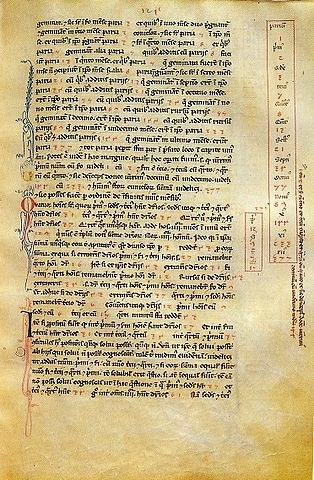
\includegraphics[width=.4\textwidth]{314px-Liber-abbaci-magliab-f124r}
\caption{A page of Fibonacci's Liber Abaci a very long title e just to prove my point more and more and more}
\source{Heinz L\"{u}neburg, Leonardi Pisani Liber Abaci oder Lesevergn\"{u}gen eines Mathematikers}
\end{figure}

\section{List of Fibonacci Numbers}

The first 11 Fibonacci numbers $F_n$ for $n = 0, 1, 2, \ldots, 10$ are:

\begin{table}[p!]\centering
\caption{First 11 Fibonacci Numbers for $n=0,1,\ldots$}
\begin{tabular}{|c|c|c|c|c|c|c|c|c|c|c|}
\hline
$F_0$ & $F_1$ & $F_2$ & $F_3$ & $F_4$ & $F_5$ & $F_6$ & $F_7$ & $F_8$ & $F_9$ & $F_{10}$\\
\hline
0 & 1 & 1 & 2 & 3 & 5 & 8 & 13 & 21 & 34 & 55 \\
\hline
\end{tabular}
\end{table}

The sequence can also be extended to negative index n using the re-arranged recurrence relation
%
\begin{equation}
F_{n-2} = F_n - F_{n-1},
\end{equation}
%
which yields the sequence of ``negafibonacci'' numbers satisfying
%
\begin{equation}
F_{-n} = (-1)^{n+1} F_n.
\end{equation}
%
Thus the bidirectional sequence is
\begin{table}[p!]\centering
\caption{Bidirectional Fibonacci Numbers sequence}
\begin{tabular}{|c|c|c|c|c|c|c|c|c|c|c|}
\hline
$F_{-5}$ & $F_{-4}$ & $F_{-3}$ & $F_{-2}$ & $F_{-1}$ & $F_0$ & $F_1$ & $F_2$ & $F_3$ & $F_4$ & $F_5$ \\\hline
5 & $-3$ & 2 & $-1$ & 1 & 0 & 1 & 1 & 2 & 3 & 5\\\hline
\end{tabular}
\end{table}

\citet{Rohl:1989} gives an account of how Fibonacci numbers can be computed efficiently.

\section{Applications}

\subsection{In Computation}

Fibonacci numbers have wide applications in mathematics as well as computer science:

\begin{itemize}
\item The Fibonacci numbers are important in the computational run-time analysis of Euclid's algorithm to determine the greatest common divisor of two integers: the worst case input for this algorithm is a pair of consecutive Fibonacci numbers.

\item Yuri Matiyasevich was able to show that the Fibonacci numbers can be defined by a Diophantine equation, which led to his original solution of Hilbert's tenth problem.

\item The Fibonacci numbers are also an example of a complete sequence. This means that every positive integer can be written as a sum of Fibonacci numbers, where any one number is used once at most.

\item Moreover, every positive integer can be written in a unique way as the sum of one or more distinct Fibonacci numbers in such a way that the sum does not include any two consecutive Fibonacci numbers. This is known as Zeckendorf's theorem, and a sum of Fibonacci numbers that satisfies these conditions is called a Zeckendorf representation. The Zeckendorf representation of a number can be used to derive its Fibonacci coding.

\item Fibonacci numbers are used by some pseudorandom number generators.

\item Fibonacci numbers are used in a polyphase version of the merge sort algorithm in which an unsorted list is divided into two lists whose lengths correspond to sequential Fibonacci numbers -- by dividing the list so that the two parts have lengths in the approximate proportion $\varphi$. A tape-drive implementation of the polyphase merge sort was described in The Art of Computer Programming.

\item Fibonacci numbers arise in the analysis of the Fibonacci heap data structure.

\item The Fibonacci cube is an undirected graph with a Fibonacci number of nodes that has been proposed as a network topology for parallel computing.

\item A one-dimensional optimization method, called the Fibonacci search technique, uses Fibonacci numbers.

\item The Fibonacci number series is used for optional lossy compression in the IFF 8SVX audio file format used on Amiga computers. The number series compands the original audio wave similar to logarithmic methods such as $\mu$-law.

\item Since the conversion factor 1.609344 for miles to kilometers is close to the golden ratio (denoted $\varphi$), the decomposition of distance in miles into a sum of Fibonacci numbers becomes nearly the kilometer sum when the Fibonacci numbers are replaced by their successors. This method amounts to a radix 2 number register in golden ratio base $\varphi$ being shifted. To convert from kilometers to miles, shift the register down the Fibonacci sequence instead.
\end{itemize}


\subsection{In Nature}

Fibonacci sequences appear in biological settings, in two consecutive Fibonacci numbers, such as branching in trees, arrangement of leaves on a stem, the fruitlets of a pineapple, the flowering of artichoke, an uncurling fern and the arrangement of a pine cone, and the family tree of honeybees. However, numerous poorly substantiated claims of Fibonacci numbers or golden sections in nature are found in popular sources, e.g.,~relating to the breeding of rabbits in Fibonacci's own unrealistic example, the seeds on a sunflower, the spirals of shells, and the curve of waves.

A model for the pattern of florets in the head of a sunflower was proposed by H.~Vogel in 1979. \cite{Vogel:1979} This has the form
\begin{equation}
\theta = \frac{2\pi}{\phi^2} n,\  r = c \sqrt{n}
\end{equation}
where $n$ is the index number of the floret and $c$ is a constant scaling factor; the florets thus lie on Fermat's spiral. 

\begin{figure}[p!]\centering
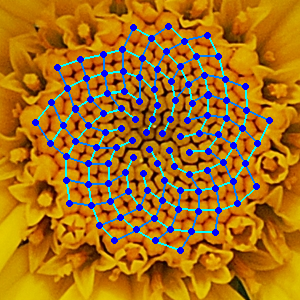
\includegraphics[width=.5\textwidth]{FibonacciChamomile}

\caption{Yellow Chamomile head}
\end{figure}